\chapter{How to Crush Sales}

This chapter is based on a School of Hard Knocks entrepreneurship interview curated by LazyingArt LLC. The exchange is short, but it has a clean structure: the speaker begins with the fact that people dislike being sold to, then builds a practical method around asking questions, discovering the buyer's real need, and offering help only when the offer fits that need. There is no blackboard mathematics in the source material, so the equations in this chapter are bookkeeping devices. They make the sequence explicit without pretending that the interview gave a formal theory.

\section{Selling Without Pressure}

The opening question is direct: how could someone crush sales in 2022? The answer does not begin with tactics, scripts, or a product demonstration. It begins with a constraint on the buyer.

\begin{equation}
\text{Most people dislike being sold to,}
\qquad
\text{but people still like to buy.}
\end{equation}

That is the central tension. Selling fails when the buyer experiences the conversation as pressure. Buying becomes possible when the buyer recognizes that a real problem may be solved. The sales process therefore has to be organized around the buyer's need, not around the seller's urge to present.

\subsection{Question \& Answer}

\paragraph{Question.}
If no one likes to be sold to, how can sales work at all?

\paragraph{Answer.}
Sales can work when the seller stops treating the interaction as persuasion first and treats it as diagnosis first. The buyer is not being asked to submit to a pitch. The buyer is being helped to clarify a need, identify a pain point, and decide whether the seller has something that genuinely addresses it.

In compact form, the first move is this:

\begin{equation}
\text{pressure on buyer}
\quad \longrightarrow \quad
\text{resistance},
\end{equation}

while the method proposed in the interview is closer to

\begin{equation}
\text{need discovered}
\quad \longrightarrow \quad
\text{solution evaluated}
\quad \longrightarrow \quad
\text{buyer chooses}.
\end{equation}

The distinction is small in words and large in practice. The seller is not trying to make the buyer want something. The seller is trying to find out what the buyer already needs.

\section{Solution Selling}

The speaker gives the method a name: solution selling. He also notes that there are many names for it, which matters. The label is not the source of the method. The sequence is.

Let \(N\) denote the buyer's true need, and let \(S\) denote a proposed solution. A seller who begins with \(S\) before discovering \(N\) is working in the wrong direction. The disciplined order is

\begin{equation}
\text{questions}
\;\longrightarrow\;
N
\;\longrightarrow\;
\text{possible fit of } S
\;\longrightarrow\;
\text{mutual problem-solving}.
\end{equation}

The phrase ``true need'' is important. It means the seller should not merely hear the first surface complaint and rush to match it with a feature. The seller asks questions until the conversation has uncovered what actually matters to the client.

\begin{definition}
A \emph{solution-selling conversation} is a sales conversation in which the seller first asks questions, then identifies the buyer's need \(N\), and only then decides whether a proposed solution \(S\) can help.
\end{definition}

This gives us a minimal fit relation:

\begin{equation}
\operatorname{Fit}(S,N)=
\begin{cases}
1, & \text{if } S \text{ helps solve } N,\\
0, & \text{if } S \text{ does not help solve } N.
\end{cases}
\end{equation}

This notation is deliberately modest. It does not claim that sales can be reduced to a formula. It simply records the logic of the interview: do not present the solution before you know what problem it is supposed to solve.

\section{Questions Before Claims}

The speaker's own description of the method is simple: he sells by asking questions, understanding the real need first, and then seeing whether he can help solve that need. The seller's first task is therefore not performance. It is inquiry.

We can write the operating rule as

\begin{equation}
\text{Ask first, claim second.}
\end{equation}

More explicitly,

\begin{align}
Q &:= \text{questions asked of the client},\\
N(Q) &:= \text{need revealed by those questions},\\
S &:= \text{seller's possible solution}.
\end{align}

The seller should move to presentation only after \(N(Q)\) is sufficiently clear. In practical language, the questions create the conditions under which the seller can know whether the offer belongs in the conversation at all.

\begin{figure}
\centering
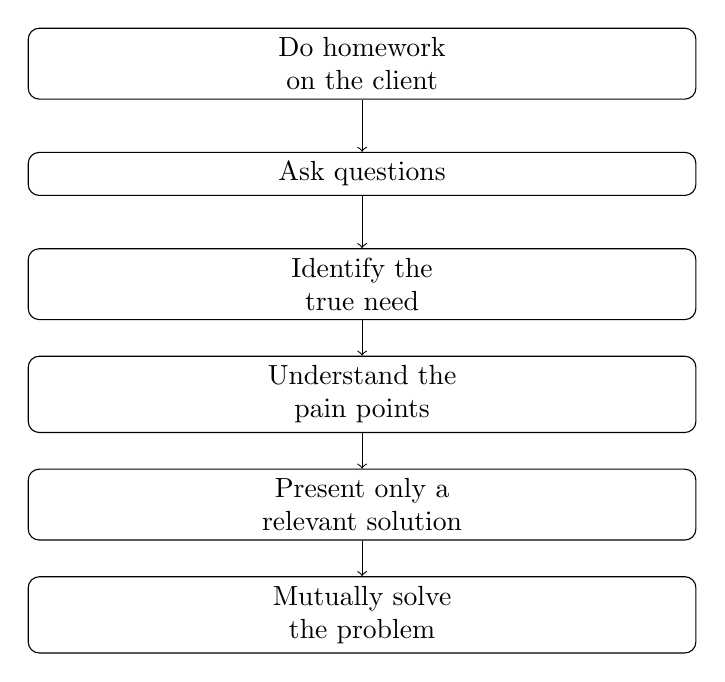
\begin{tikzpicture}
\node[draw, rounded corners, align=center, text width=0.68\linewidth] (a) at (0,0) {Do homework\\on the client};
\node[draw, rounded corners, align=center, text width=0.68\linewidth] (b) at (0,-1.4) {Ask questions};
\node[draw, rounded corners, align=center, text width=0.68\linewidth] (c) at (0,-2.8) {Identify the\\true need};
\node[draw, rounded corners, align=center, text width=0.68\linewidth] (d) at (0,-4.2) {Understand the\\pain points};
\node[draw, rounded corners, align=center, text width=0.68\linewidth] (e) at (0,-5.6) {Present only a\\relevant solution};
\node[draw, rounded corners, align=center, text width=0.68\linewidth] (f) at (0,-7.0) {Mutually solve\\the problem};
\draw[->] (a) -- (b);
\draw[->] (b) -- (c);
\draw[->] (c) -- (d);
\draw[->] (d) -- (e);
\draw[->] (e) -- (f);
\end{tikzpicture}
\caption{A transcript-derived flow of the solution-selling method. No retained frame shows this as a board diagram; it is a compact reconstruction of the spoken sequence.}
\end{figure}

\section{The Demo-First Failure Mode}

The speaker then turns to the opposite method. A young salesperson comes in and says, in effect: let me do a demo, let me show you everything I have, and stop me when you see something interesting. The criticism is that this makes the buyer do the diagnostic work.

In the notation above, demo-first selling starts with \(S\) and hopes to stumble into \(N\):

\begin{equation}
S_1,S_2,S_3,\ldots
\quad \text{shown before} \quad
N \text{ is known}.
\end{equation}

That is not discovery. It is random search. The buyer is forced to scan the seller's inventory and decide whether any part of it happens to matter.

A compact comparison helps keep the contrast clear:

\begin{table}
\centering
\begin{tabular}{p{0.42\linewidth}p{0.42\linewidth}}
\textbf{Demo-first selling} & \textbf{Solution selling} \\
Starts with what the seller has & Starts with what the buyer needs \\
Shows many features early & Asks questions early \\
Waits for interest to appear & Diagnoses pain points first \\
Treats fit as accidental & Tests fit deliberately \\
Feels like pressure & Can feel like help \\
\end{tabular}
\caption{The lecture's main contrast: product-centered demonstration versus need-centered diagnosis.}
\end{table}

The speaker's rough image is that the demo-first method throws things at the wall to see what sticks. The point is not merely that the method is inelegant. It is that the seller has not earned the right to know what should be shown.

\section{Homework, Pain Points, And Fit}

After rejecting the random demo, the speaker pivots: slow down. Do the homework on the client before showing up. He adds that few people do this, which turns preparation into an advantage.

Let \(H\) denote the seller's homework, and let \(P\) denote the client's pain points. The useful sequence is

\begin{equation}
H
\;\longrightarrow\;
P
\;\longrightarrow\;
N
\;\longrightarrow\;
\operatorname{Fit}(S,N).
\end{equation}

This is not a separate theory from solution selling. It is the operational form of it. Homework helps the seller ask better questions. Better questions reveal sharper pain points. Sharper pain points make it possible to test whether the proposed solution actually belongs.

\subsection{A Worked Fit Check}

Suppose the seller has a set of possible features

\begin{equation}
S=\{s_1,s_2,s_3\},
\end{equation}

and the client conversation reveals two pain points,

\begin{equation}
P=\{p_1,p_2\}.
\end{equation}

The demo-first seller presents \(s_1,s_2,s_3\) and waits. The solution seller instead asks which elements of \(S\) address \(P\). The relevant working table is the fit map

\begin{equation}
F_{ij}=
\begin{cases}
1, & \text{if feature } s_i \text{ helps with pain point } p_j,\\
0, & \text{otherwise.}
\end{cases}
\end{equation}

A disciplined seller presents the parts of \(S\) for which at least one \(F_{ij}=1\). The seller withholds, postpones, or discards the parts that do not touch the client's pain.

The update rule is therefore

\begin{equation}
S_{\text{present}}
=
\{\,s_i \in S : \text{there exists } p_j \in P
\text{ with } F_{ij}=1\,\}.
\end{equation}

This is only a clean notation for the transcript's practical advice: talk to the client about their pain points and solve a problem together, rather than trying to sell from a pile of unrelated offerings.

\section{Mutual Problem-Solving}

The last movement of the lecture is ethical and commercial at the same time. The seller should talk with the client about the pain points and mutually solve a problem. That word ``mutually'' matters. It changes the posture of the interaction.

The seller is not a pusher of inventory. The seller is a participant in a problem-solving process. In symbols,

\begin{equation}
\text{sale as pressure}
\neq
\text{sale as joint solution}.
\end{equation}

The difference is visible in the direction of attention. Pressure selling asks, ``How do I get this buyer to take what I have?'' Solution selling asks, ``What is the buyer trying to solve, and can I help?''

That is why the chapter belongs not only in a sales discussion, but in the broader entrepreneurship book. A business earns durable revenue when it understands the client's problem well enough to become useful. Selling, in this sense, is not separate from judgment. It is judgment under commercial pressure.

\section{Summary}

The lecture gives a short but complete sales model. Start with the buyer's resistance to being sold. Preserve the fact that the buyer still wants to buy when a real need is met. Then use questions, homework, and pain-point discovery to decide whether a solution fits.

The compact spine is

\begin{equation}
\text{homework}
\;\longrightarrow\;
\text{questions}
\;\longrightarrow\;
\text{true need}
\;\longrightarrow\;
\text{fit}
\;\longrightarrow\;
\text{mutual solution}.
\end{equation}

The rejected path is equally important:

\begin{equation}
\text{demo everything}
\;\longrightarrow\;
\text{hope something sticks}
\;\longrightarrow\;
\text{weak selling}.
\end{equation}

The practical lesson is that strong selling is not louder persuasion. It is better diagnosis.